%%
%% This is file `sample-sigconf.tex',
%% generated with the docstrip utility.
%%
%% The original source files were:
%%
%% samples.dtx  (with options: `sigconf')
%% 
%% IMPORTANT NOTICE:
%% 
%% For the copyright see the source file.
%% 
%% Any modified versions of this file must be renamed
%% with new filenames distinct from sample-sigconf.tex.
%% 
%% For distribution of the original source see the terms
%% for copying and modification in the file samples.dtx.
%% 
%% This generated file may be distributed as long as the
%% original source files, as listed above, are part of the
%% same distribution. (The sources need not necessarily be
%% in the same archive or directory.)
%%
%% Commands for TeXCount
%TC:macro \cite [option:text,text]
%TC:macro \citep [option:text,text]
%TC:macro \citet [option:text,text]
%TC:envir table 0 1
%TC:envir table* 0 1
%TC:envir tabular [ignore] word
%TC:envir displaymath 0 word
%TC:envir math 0 word
%TC:envir comment 0 0
%%
%%
%% The first command in your LaTeX source must be the \documentclass command.
\documentclass[sigconf,nonacm]{acmart}
%% NOTE that a single column version may be required for 
%% submission and peer review. This can be done by changing
%% the \doucmentclass[...]{acmart} in this template to 
%% \documentclass[manuscript,screen]{acmart}
%% 
%% To ensure 100% compatibility, please check the white list of
%% approved LaTeX packages to be used with the Master Article Template at
%% https://www.acm.org/publications/taps/whitelist-of-latex-packages 
%% before creating your document. The white list page provides 
%% information on how to submit additional LaTeX packages for 
%% review and adoption.
%% Fonts used in the template cannot be substituted; margin 
%% adjustments are not allowed.
%%
%%
%% \BibTeX command to typeset BibTeX logo in the docs
\AtBeginDocument{%
  \providecommand\BibTeX{{%
    \normalfont B\kern-0.5em{\scshape i\kern-0.25em b}\kern-0.8em\TeX}}}

%% Rights management information.  This information is sent to you
%% when you complete the rights form.  These commands have SAMPLE
%% values in them; it is your responsibility as an author to replace
%% the commands and values with those provided to you when you
%% complete the rights form.
\setcopyright{acmcopyright}
\copyrightyear{2022}
\acmYear{2022}
\acmDOI{XXXXXXX.XXXXXXX}

%% These commands are for a PROCEEDINGS abstract or paper.
\acmConference[SCORES'22]{Student Computing Research Symposium}{October 6,
2022}{Ljubljana, Slovenia}
%
%  Uncomment \acmBooktitle if th title of the proceedings is different
%  from ``Proceedings of ...''!
%
%\acmBooktitle{Woodstock '18: ACM Symposium on Neural Gaze Detection,
%  June 03--05, 2018, Woodstock, NY} 
\acmPrice{15.00}
\acmISBN{978-1-4503-XXXX-X/18/06}


%%
%% Submission ID.
%% Use this when submitting an article to a sponsored event. You'll
%% receive a unique submission ID from the organizers
%% of the event, and this ID should be used as the parameter to this command.
%%\acmSubmissionID{123-A56-BU3}

%%
%% For managing citations, it is recommended to use bibliography
%% files in BibTeX format.
%%
%% You can then either use BibTeX with the ACM-Reference-Format style,
%% or BibLaTeX with the acmnumeric or acmauthoryear sytles, that include
%% support for advanced citation of software artefact from the
%% biblatex-software package, also separately available on CTAN.
%%
%% Look at the sample-*-biblatex.tex files for templates showcasing
%% the biblatex styles.
%%

%%
%% The majority of ACM publications use numbered citations and
%% references.  The command \citestyle{authoryear} switches to the
%% "author year" style.
%%
%% If you are preparing content for an event
%% sponsored by ACM SIGGRAPH, you must use the "author year" style of
%% citations and references.
%% Uncommenting
%% the next command will enable that style.
%%\citestyle{acmauthoryear}

\newcommand{\scores}{\textsc{SCORES}}
\renewcommand{\keywordsname}{Ključne besede}
\renewcommand{\acksname}{Zahvala}

\usepackage[slovene]{babel}
\usepackage{verbatim}
\usepackage{booktabs}
\usepackage{float}
\usepackage[linesnumbered, boxed, resetcount]{algorithm2e}
\SetAlgorithmName{Algoritem}{Algoritem}

%%
%% If you need any other LaTeX packages, add them here
%%

%%
%% end of the preamble, start of the body of the document source.
\begin{document}

%%
%% The "title" command has an optional parameter,
%% allowing the author to define a "short title" to be used in page headers.
\title{Optimizacija več-agentnega iskanja poti z uvedbo lokalnih vodij}

%%
%% The "author" command and its associated commands are used to define
%% the authors and their affiliations.
%% Of note is the shared affiliation of the first two authors, and the
%% "authornote" and "authornotemark" commands
%% used to denote shared contribution to the research.
\author{Andraž Šošterič}
%\authornote{Vsi trije avtorji so prispevali enakovreden dele\v{z}.}
\email{andraz.sosteric@student.um.si}
\affiliation{%
    \institution{Faculty of Electrical \\Engineering and Computer Science,\\
    University of Maribor\\Koroška cesta 46}
    \city{SI-2000 Maribor}
    \country{Slovenia}
}

\author{David Lipavec}
%\authornotemark[1]
\email{david.lipavec@student.um.si}
\affiliation{%
    \institution{Faculty of Electrical \\Engineering and Computer Science,\\
    University of Maribor\\Koroška cesta 46}
    \city{SI-2000 Maribor}
    \country{Slovenia}
}

\author{Nejc Fras}
%\authornotemark[1]
\email{nejc.fras@student.um.si}
\affiliation{%
    \institution{Faculty of Electrical \\Engineering and Computer Science,\\
    University of Maribor\\Koroška cesta 46}
    \city{SI-2000 Maribor}
    \country{Slovenia}
}

\author{Tadej Teršek}
%\authornotemark[1]
\email{tadej.tersek@student.um.si}
\affiliation{%
    \institution{Faculty of Electrical \\Engineering and Computer Science,\\
    University of Maribor\\Koroška cesta 46}
    \city{SI-2000 Maribor}
    \country{Slovenia}
}

%%
%% Keywords. The author(s) should pick words that accurately describe
%% the work being presented. Separate the keywords with commas.
\keywords{centralizirano načrtovanje poti, distribuirano načrtovanje poti, usklajevanje agentov, izogibanje trkom, optimizacija poti}

%%
%% This command processes the author and affiliation and title
%% information and builds the first part of the formatted document.
\maketitle

\section{Uvod}

V tem članku obravnavamo problem več-agentnega iskanja poti (Multi-Agent Path Finding / MAPF), 
ki se v praksi pojavlja v številnih domenah, kot so robotizirana skladišča, avtonomna vozila, 
inteligentni transportni sistemi in drugi logistični sistemi. Gre za temeljni problem koordinacije 
več avtonomnih enot v skupnem prostoru, kjer mora vsak agent doseči svoj cilj brez trkov z 
drugimi agenti ali ovirami.

Cilj problema je načrtovati poti za množico agentov v diskretnem prostoru tako, da se izognemo 
medsebojnim konfliktom in hkrati optimiziramo določene metrike, kot sta skupni čas izvajanja 
(ang. \textit{makespan}) ali vsota dolžin poti (ang. \textit{sum of costs})~\cite{stern2019multiagent}.

Repozitorij z izvorno kodo projekta je na voljo na našem github repozitoriju~\footnote{\url{https://github.com/Asos75/MultiAgent}}.

V nadaljevanju bomo primerjali centralizirane metode, katerih predstavnika sta LaCAM in PBS, 
ki načrtujejo poti za vse agente z uporabo globalnega pogleda na problem, ter decentralizirane 
pristope, kot sta Follower in MATS-LP, kjer posamezni agenti sprejemajo odločitve lokalno brez 
centralnega nadzora in imajo pregled le nad svojo okolico.

Na ta način bomo analizirali ključne razlike med obema paradigmama z vidika učinkovitosti, 
skalabilnosti in kakovosti rešitev. Centralizirani pristopi praviloma zagotavljajo bolj 
optimalne rešitve, vendar slabše skalirajo z naraščajočim številom agentov, medtem ko 
decentralizirani pristopi omogočajo boljšo razširljivost, vendar pogosto na račun kakovosti 
rešitev.

Kot glavni referenčni algoritem izberemo delo 
\textit{LaCAM: Search-Based Algorithm for Quick Multi-Agent Pathfinding}~\cite{okumura2023lacam}, 
ki predstavlja sodoben in učinkovit centraliziran pristop k reševanju problema MAPF. Izbrani 
članek služi kot referenčna osnova za našo analizo, saj ponuja dobro ravnovesje med 
učinkovitostjo in skalabilnostjo ter omogoča relativno enostavno reprodukcijo eksperimentov.

LaCAM bomo uporabili kot predstavnika centraliziranih metod, s katerim bomo primerjali 
decentralizirane pristope, kot sta Follower in MATS-LP, ter tako sistematično analizirali 
razlike med globalnim in lokalnim načrtovanjem poti.

\subsection{Definicija problema}

Stern et al.~\cite{stern2019multiagent} definirajo problem več-agentnega iskanja poti (Multi-Agent Path Finding - MAPF)
 kot trojico
\[
\langle G, s, t \rangle,
\]
kjer je \( G = (V, E) \) neusmerjen graf, pri čemer \( V \) predstavlja množico vozlišč, \( E \) 
pa množico povezav.

\vspace{0.5em}
\noindent Podana je množica agentov \( A = \{1, 2, \dots, k\} \). Funkcija
\[
s : \{1, \dots, k\} \rightarrow V
\]
preslika vsakega agenta v njegovo začetno vozlišče, funkcija
\[
t : \{1, \dots, k\} \rightarrow V
\]
pa v njegovo ciljno vozlišče.

\vspace{0.5em}
\noindent Naj bo $\pi_i[t]\in V$ položaj agenta $i$ v diskretnem času $t\in\mathbb{N}_{\ge 0}$. Pri vsakem koraku $t$ se agent $i$ lahko 
premakne v sosednje vozlišče ali ostane na trenutnem, tj.
\[\pi_i[t+1]\in\mathrm{neigh}(\pi_i[t])\cup\{\pi_i[t]\},\]
kjer je $\mathrm{neigh}(v)$ množica vozlišč, sosednjih vozlišču $v\in V$~\cite{okumura2023lacam}.

\vspace{0.5em}
\noindent 
Po Okamuri~\cite{okumura2023lacam} se mora agent izogibati naslednjim vrstam konfliktov:

\begin{itemize}
    \item \textbf{Vozliščni konflikt:} Do vozliščnega konflikta (ang. vertex conflict) pride, če nameravata $ \pi_i $ in $ \pi_j $ zasedeti isto 
    vozlišče v istem trenutku, torej obstaja časovni korak $t$, da velja $ \pi_i[t] = \pi_j[t] $.~\cite{stern2019multiagent}
    \item \textbf{Zamenjalni konflikt:} Do zamenjalnega konflikta (ang. swap conflict) pride, če nameravata $ \pi_i $ in $ \pi_j $ zamenjati svoji
    poziciji v istem trenutku, torej obstaja časovni korak $t$, da velja $ \pi_i[t] = \pi_j[t+1] \wedge \pi_i[t+1] = \pi_j[t] $~\cite{stern2019multiagent}.
\end{itemize}

\vspace{0.5em}
\noindent 
Rešitev MAPF za instance, omenjene zgoraj, je množica brezkonfliktnih poti
 $\{\pi_1,\ldots,\pi_k\}$ takih, da obstaja časovni korak $T \in \mathbb{N}_{\ge 0}$, kjer agent doseže cilj.~\cite{okumura2023lacam}
 
\section{Sorodna dela}

V tem razdelku izpostavimo ključna dela s področja več-agentnega iskanja poti, 
ki dopolnjujejo in razširjajo pogled iz uvoda. Pri vsakem delu na kratko povemo,
kaj je njegova glavna ideja in kakšen doprinos ima k našemu eksperimentu.

\subsection{Centralizirani pristopi}


	\textit{EECBS}~\cite{li2021eecbs} je nadgradnja klasičnega CBS, ki ohrani dvonivojsko iskanje, hkrati pa z
    \textit{Explicit Estimation Search} in uteževanjem omogoča nadzorovano suboptimalnost (uporabnik nastavi 
    kompromis med kakovostjo in časom). Avtorji poročajo o bistveno boljši skalabilnosti na večjih instancah 
    ob majhni, dokazljivo omejeni degradaciji kakovosti rešitve. EECBS uporabimo kot referenčno izhodišče za 
    razumevanje kompromisa »hitrost vs. kvaliteta« pri centraliziranih metodah; njegove ideje utemeljijo, zakaj 
    v evalvaciji poleg kakovosti (SoC/makespan) spremljamo tudi čas izvajanja in skalabilnost.


	\textit{CBSH2}~\cite{li2019disjoint} izboljša CBS z močnejšimi hevristikami in tehniko \textit{disjoint splitting}, 
    ki z uvedbo pozitivnih omejitev zmanjša podvajanje iskanja in s tem velikost iskalnega drevesa. Rezultat je 
    hitrejše reševanje in boljša skalabilnost ob ohranjeni rešitveni kakovosti tipične za CBS-družino. CBSH2 obravnavamo 
    kot dodatno referenco znotraj centraliziranih metod, ki pokaže, da so izboljšave pogosto posledica boljšega 
    upravljanja konfliktov; to nam pomaga pri interpretaciji rezultatov LaCAM/PBS (kjer tudi ciljamo na učinkovitejšo 
    obravnavo konfliktov), če opazimo razlike predvsem v času in ne v SoC.

\subsection{Decentralizirani pristopi}


	\textit{Follower}~\cite{andreychuk2024follower} je decentraliziran pristop za \textit{lifelong} MAPF, ki 
    kombinira (i) hevristični planer (npr. A* nad statičnimi ovirami), ki generira »razpršene« poti z namenom 
    zmanjšanja zasičenosti ozkih grl, in (ii) naučeno politiko sledenja, ki lokalno reagira na druge agente in 
    se izogiba trkom. Izvajanje je povsem lokalno (brez centralnega koordinatorja), zato metoda dobro skalira, 
    vendar je kakovost poti odvisna od lokalnih informacij in stabilnosti naučene politike. Follower je eden 
    naših glavnih decentraliziranih primerjalnih algoritmov; z njim ovrednotimo, kako se učeni, lokalni pristopi 
    primerjajo s centraliziranima LaCAM/PBS in z našim hibridnim pristopom z lokalnimi vodji.

	\textit{Decentralized Monte Carlo Tree Search for Partially Observable Multi-agent Pathfinding}~\cite{skrynnik2024mcts} 
    predlaga decentralizirano reševanje \textit{lifelong} MAPF pri delni opazljivosti: vsak agent iz lokalnih opazovanj 
    zgradi intrinzični (lokalni) MDP in na njem izvaja MCTS, ki ga dodatno usmerja nevronska politika. S simulacijami v 
    drevesu agenti ocenjujejo kratkoročne interakcije z bližnjimi agenti, koordinacija pa nastaja implicitno (brez 
    eksplicitne komunikacije ali centralnega koordinatorja), kar vodi do dobre skalabilnosti. delo utemeljuje našo 
    izbiro decentraliziranih primerjalnih metod na POGEMA (delna opazljivost) in je neposredno relevantno za komponento 
    MATS-LP v naši primerjavi, kjer želimo videti, ali »lookahead« (MCTS) izboljša pretočnost in robustnost glede na 
    bolj reaktivne politike.

	\textit{PRIMAL2}~\cite{damani2021primal2} je zgodnje, vplivno delo, ki pokaže, da je mogoče MAPF reševati z 
    decentraliziranimi politikami na osnovi lokalnih opazovanj, naučenimi s kombinacijo \textit{imitation learning} 
    (iz centraliziranih planerjev) in \textit{reinforcement learning}. Pristop zelo dobro skali, vendar pogosto žrtvuje 
    optimalnost in lahko povzroča neusklajenosti v gostih scenarijih. PRIMAL2 
    uporabljamo kot kontekst za interpretacijo rezultatov učenih decentraliziranih metod (Follower/MATS-LP/SCRIMP): če 
    pri njih opazimo slabši SoC, je to pričakovan trade-off, ki ga literatura že izpostavlja.

	\textit{SCRIMP}~\cite{wang2023scrimp} uvede eksplicitno komunikacijo med agenti z uporabo transformer arhitekture in 
    pozornostnega mehanizma, kar omogoča učinkovitejšo koordinacijo tudi pri zelo omejenem vidnem polju. S tem pristop 
    preseže omejitve povsem nekomunikacijskih lokalnih politik, hkrati pa ohrani decentralizirano izvajanje in dobro skalabilnost. 
    SCRIMP služi kot motivacija za naš »hibridni« pogled (lokalni vodje): kaže, da lahko 
    dodaten koordinacijski signal (komunikacija ali posredno usklajevanje) izboljša pretočnost; naš pristop to doseže z lažjim 
    mehanizmom vodij, ki ga lahko primerjamo z relacijo med čisto lokalnimi in bolj koordiniranimi pristopi.

\subsection{Primerjalne platforme}

	\textit{POGEMA}~\cite{skrynnik2025pogema} ponuja standardizirano platformo za evalvacijo MAPF algoritmov v (delno) opazljivih 
    okoljih, z generatorjem instanc in enotnimi metrikami ter protokolom izvajanja. Omogoča pošteno in ponovljivo primerjavo 
    različnih pristopov. POGEMA je naše glavno evalvacijsko ogrodje, zato se metodologija, metrike in primerjava rezultatov 
    neposredno opirajo na to delo.

\section{Metodologija}

V tem poglavju bomo predstavili metodologijo vrednotenja in primerjanja izbranih algoritmov za problem večagentnega iskanja poti.
Cilj eksperimentalnega dela je primerjati centralizirane pristope, kot sta LaCAM in PBS, z decentraliziranimi pristopi Follower 
in MATS-LP ter ovrednotiti predlagani hibridni pristop z lokalnimi vodji.

\subsection{Experimentalno okolje}

Za primerjalno okolje bomo uporabili knjižnico POGEMA~\cite{skrynnik2025pogema}, ki omogoča standardizirano evalvacijo MAPF
algoritmov v delno opazljivih okoljih, ter to kombinirali z MovingAI~\cite{stern2019multiagent} knjižnico zemljevidov za testiranje agentov.

POGEMA je dostopna kot standardna Python knjižnica, medtem ko so implementacije posameznih algoritmov pridobljene iz uradnih repozitorijev 
avtorjev izbranih člankov. Ker različni algoritmi uporabljajo različne vhodne formate in interne predstavitve okolja, je bilo potrebno za 
vsako implementacijo razviti poseben prilagoditveni sloj (\textit{adapter}), ki omogoča vključitev algoritma v skupno evalvacijsko ogrodje.

\subsection{Metrike}

\textbf{Sum-of-Costs (SoC)} je vsota časovnih korakov, ki jih vsi agenti porabijo za dosego svojih ciljnih vozlišč~\cite{stern2019multiagent}:
\[
    \text{SoC} = \sum_{i=1}^{k} |\pi_i|,
\]
kjer je $|\pi_i|$ dolžina poti agenta $i$. Nižja vrednost pomeni učinkovitejšo
rešitev. 
\vspace{0.5em}

SoC je ena izmed najpogosteje uporabljenih metrik v MAPF literaturi~\cite{stern2019multiagent}, kar omogoča neposredno primerjavo z obstoječimi deli. 
Metrika meri skupni strošek kot vsoto dolžin poti vseh agentov in s tem neposredno zajame celostno učinkovitost sistema.

Metrika je še posebej primerna za one-shot scenarije, saj minimizacija SoC ustreza cilju minimizacije skupne porabe časa oziroma virov. Hkrati 
kaznuje neučinkovite poti posameznih agentov, kar spodbuja iskanje globalno učinkovitih rešitev. SoC bomo zato uporabili za vrednotenje algoritmov 
LaCAM in PBS na zbirki MovingAI.

\vspace{0.5em}
\noindent
\textbf{Makespan} je čas, ki ga porabi najdaljša pot med vsemi agenti, torej
maksimum nad vsemi $|\pi_i|$~\cite{stern2019multiagent}:
\[
    \text{makespan} = \max_{i \in \{1,\dots,k\}} |\pi_i|.
\]

Metrika odraža skupno trajanje reševanja instance in je primerna za scenarije, kjer je ključen vzporedni zaključek vseh agentov. Makespan je 
uveljavljena metrika v MAPF literaturi~\cite{stern2019multiagent} in je še posebej relevantna v praktičnih aplikacijah, kjer je ključen vzporedni 
zaključek vseh agentov. 

Makespan je pri primerjavi centraliziranih algoritmov nujna dopolnitev k SoC, saj sama vsota stroškov namreč ne razkrije, ali posamezen agent 
morda bistveno zavlačuje celotno skupino. Z vključitvijo obeh metrik tako dobimo celovitejšo in bolj zanesljivo oceno učinkovitosti algoritma v realnih pogojih.

\vspace{0.5em}
\noindent
\textbf{Stopnja uspeha (Success Rate)} meri delež instanc, pri katerih vsi
agenti uspešno dosežejo svoje cilje znotraj predvidenega časovnega
horizonta~\cite{skrynnik2025pogema}. 

Stopnja uspeha je primarna metrika platforme POGEMA in skupaj s pretokom (ang.\ throughput) tvori osnovo za vrednotenje na tej platformi~\cite{skrynnik2025pogema}. 
Zasnovana je posebej za vrednotenje decentraliziranih metod v delno opazljivih okoljih. Metrika je za naš eksperiment ključna, saj za razliko od SoC in makespana meri tudi 
robustnost algoritma oziroma njegovo sposobnost, da instanco v celoti reši kljub omejenim lokalnim opazovanjem.

\vspace{0.5em}
\noindent
\textbf{Čas načrtovanja} merimo kot skupni čas izvajanja algoritma na
posamezni instanci. Ta metrika je še posebej pomembna pri primerjavi med kategorijama, saj centralizirani načrtovalec tipično porabi več časa za globalno načrtovanje, 
kot decentralizirani agenti. 

Čas načrtovanja je v praktičnih aplikacijah enako pomemben kot kakovost rešitve, saj algoritem z optimalno potjo, a dolgim časom načrtovanja, v realnih sistemih ni uporaben. 
Ta metrika nam tako omogoča primerjavo med pristopoma z vidika razširljivosti in praktične uporabnosti.

\subsection{Protokol primerjave}
Primerjavo bomo izvedli na dveh ravneh:
\begin{enumerate}
    \item \textbf{Znotraj kategorije:} LaCAM in PBS primerjamo na 
    MovingAI zbirki po metrikah SoC, makespan in čas načrtovanja. 
    Follower in MATS-LP primerjamo na POGEMA zbirki po metrikah 
    throughput in stopnja uspeha.
    
    \item \textbf{Med kategorijama na skupni zbirki:} Obe katergoriji 
    bomo primerjali med seboj na skupni zbirki, kjer bomo primerjali 
    prej navedene metrike.
\end{enumerate}

\subsection{Uvedba lokalnih vodij}

Glavni prispevek tega dela je predlagana nadgradnja obstoječih pristopov, ki uvaja koncept 
\textit{lokalnih vodij}. Gre za hibridni algoritem \textit{Local Leaders}, ki združuje prednosti
centraliziranega in decentraliziranega pristopa. Algoritem je povsem
\textit{online} -- brez vnaprejšnjega načrtovanja -- in deluje v petih korakih
pri vsakem časovnem koraku~(sl.~\ref{fig:flowchart}).

\begin{figure}[H]
    \centering
    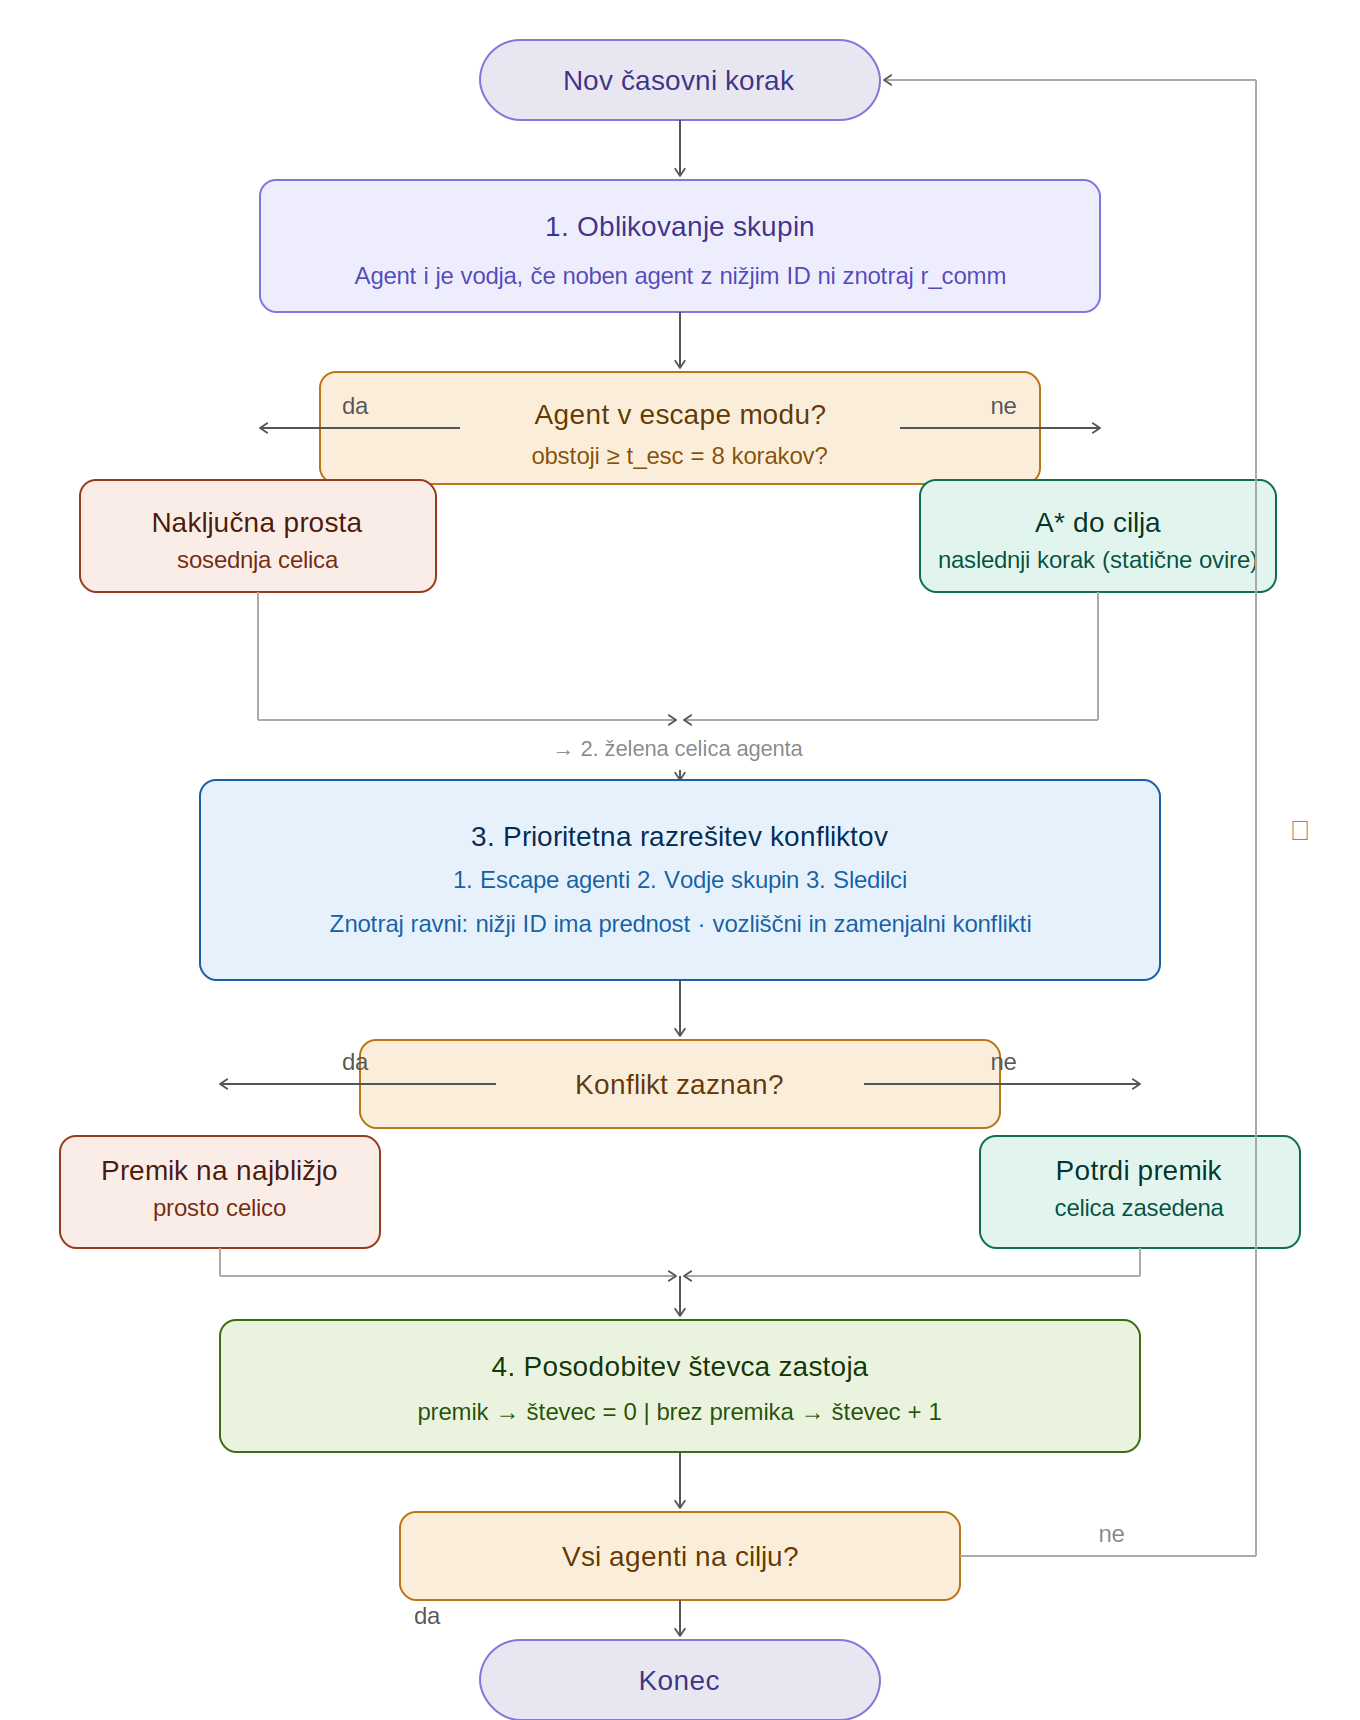
\includegraphics[width=\linewidth]{../latex/slike/flowchart_local_leaders.png}
    \caption{Diagram poteka algoritma Local Leaders: dinamično oblikovanje skupin,
    določitev vodje, A* načrtovanje in prioritetna razrešitev konfliktov.}
    \label{fig:flowchart}
\end{figure}

\paragraph{1. Oblikovanje skupin.}
Na začetku vsakega koraka, se agenti razdelijo v skupine. Pravilo za deljenje je preprosto in
deterministično: Agent $i$ postane \textit{vodja}, če nobeden od agentov z nižjim ID-jem ne 
leži znotraj razdalje $r_{\text{comm}}$ (Manhattan). Procesiranje agentov, od najnižjega do
najvišjega ID-ja zagotovi konsistentno particijo brez dvoumnosti.

\textbf{Ključna lastnost}: particija se spremeni vsak korak, tako da je članstvo v skupini
dinamično glede na trenutno postaavitev.

\paragraph{2. Željena celica (A*).}
Vsak agent zase neodvisno izvede algoritem A* od svojega položaja, do cilja pri čimer gleda le
na statične ovire. Agent na tej točki ignorira ostale agente. Rezultat tega koraka, je prva celica
najkrajše poti, to je celica kamor se agent \textit{želi} premakniti. Agenti, ki so obstali 
$\geq t_{\text{esc}}$ korakov (\textit{escape mode}), namesto A* izberejo naključno prosto 
sosednje celico, s čimer prekinejo tesnobne zastoje v hodnikih.

\paragraph{3. Prioritetna razrešitev konfliktov.}
Agenti se obdelajo v vrstnem redu prioritet:
\begin{enumerate}
    \item agenti v escape modu (najvišja prioriteta),
    \item vodje skupin,
    \item sledilci.
\end{enumerate}
Znotraj vsake ravni je prednost pri agentih z nižjim ID-jem. Za vsakega agenta
se preverita \textit{vozliščni} in \textit{zamenjalni} konflikt. V primeru
konflikta se agent pomakne v najbližjo prosto, še nezaseženo celico. Ker se
agenti z višjo prioriteto potrdijo prej, nižjeprioritentni agenti vedno vidijo
zasedene celice in se jim izognejo, tako se izognemo konfliktom v fizikalnem koraku.

\paragraph{4. Posodobitev števca zastoja.}
Agent, ki se ni premaknil, poveča števec zastoja; agent, ki se je premaknil,
ga ponastavi na nič.

\paragraph{5. Implementacija.}
Algoritem je implementiran v Pythonu za integracijo z okoljem POGEMA in MovingAI, ter v C++ 
(prek pybind11) za hitrejše izvajanje. Parametri uporabljeni za testiranje so $r_{\text{comm}} = 7$, $t_{\text{esc}} = 8$.

Lokalni vodja nima globalnega pogleda nad celotnim okoljem, temveč razpolaga le z
informacijami o agentih znotraj svoje skupine in njihove neposredne okolice.
Na ta način se bistveno zmanjša kompleksnost načrtovanja v primerjavi s centraliziranimi
algoritmi, hkrati pa se ohrani višja stopnja koordinacije kot pri popolnoma
decentraliziranih pristopih.

Hipoteza našega dela je, da lahko takšen hibridni pristop doseže boljše razmerje med
kakovostjo rešitev in časom načrtovanja kot obstoječi centralizirani ali decentralizirani
pristopi posebej. Pričakujemo nižji \textit{makespan} in višjo stopnjo uspeha kot pri
decentraliziranih metodah ter bistveno krajši čas načrtovanja kot pri popolnoma
centraliziranih algoritmih.

\section{Eksperiment in analiza rezultatov}

Po začetni validaciji implementacij smo zasnovali lasten eksperiment, ki bo primerjal centralizirane,
decentralizirane in hibridni pristop z lokalnimi vodji. Namen experimenta je preveriti ali lahko uvedba
lokalnih vodij izboljša razmerje med kakovostjo rešitev in časom načrtovanja.

Experimente izvajamo na standardiziranih zemlevidih iz zbirk MovingAI in POGEMA, na različnih velikostih 
zemljevidov, gostotah agentov in scenarijih. Tu so najbolj zanimivi scenariji z visoko gostoto agentov, 
kjer se razlike med rešitvami najbolj pokažejo.

\subsubsection{Testne instance}

Uporabljamo tri glavne tipe okolij:

\begin{itemize}
    \item \textbf{Odprte mreže} (\textit{random grids}) – okolja z malo ovirami, kjer 
    je večina konfliktov posledica visoke gostote agentov.
    
    \item \textbf{Labirinti} (\textit{mazes}) – okolja z ozkimi prehodi in številnimi lokalnimi ozkimi 
    grli, kjer je koordinacija agentov bistveno zahtevnejša.
    
    \item \textbf{Skladiščni scenariji} (\textit{warehouse maps}) – realistične postavitve, podobne 
    robotiziranim skladiščem, kjer se agenti pogosto srečujejo na križiščih in v ozkih hodnikih.
\end{itemize}

Za vsako vrsto okolja izvajamo eksperimente pri različnih številih agentov (od 20 do 1000 agentov, odvisno od 
velikosti zemljevida), z različnimi konfiguracijami. Vsaka konfiguracija se izvede večkrat z različnimi scenariji, 
ki vključujejo začetne in ciljne pozicije agentov, rezultati pa se povprečijo, da zmanjšamo vpliv posameznih 
naključnih primerov.

\subsubsection{Primerjalni kriteriji}

Primerjavo izvajamo med tremi kategorijami pristopov:

\begin{enumerate}
    \item \textbf{Centralizirani pristopi} (LaCAM, PBS),
    \item \textbf{Decentralizirani pristopi} (Follower, MATS-LP),
    \item \textbf{Hibridni pristop} (lokalni vodje).
\end{enumerate}

Za vse metode spremljamo naslednje metrike:

\begin{itemize}
    \item \textbf{SoC},
    \item \textbf{makespan},
    \item \textbf{stopnja uspeha},
    \item \textbf{čas načrtovanja}.
\end{itemize}

Pri decentraliziranih metodah dodatno spremljamo tudi \textit{throughput}, saj je ta metrika posebej pomembna pri lifelong MAPF scenarijih.

Posebej nas zanima:

\begin{itemize}
    \item kako hitro začne kakovost centraliziranih metod padati zaradi časovne zahtevnosti,
    \item pri kateri gostoti agentov decentralizirani pristopi izgubijo stabilnost,
    \item ali hibridni pristop uspe ohraniti dobro kakovost rešitev ob bistveno krajšem času načrtovanja.
\end{itemize}

\subsection{Rezulatati}

\bibliographystyle{ACM-Reference-Format}
\bibliography{bibliografija}

\end{document}
